\documentclass[paper=a4, fontsize=11pt]{scrartcl}

\usepackage{graphicx}
\usepackage{listings}
\usepackage{caption}
\usepackage{subcaption}
\usepackage{xcolor}
\usepackage{amsmath}
\usepackage{pgfplots}


\lstset{language=C++,
		backgroundcolor=\color{black!5}
}

%%% Custom sectioning
\usepackage{sectsty}
\allsectionsfont{\centering \scshape}


%%% Maketitle metadata
\newcommand{\horrule}[1]{\rule{\linewidth}{#1}} 	% Horizontal rule

\title{
	\horrule{0.5pt} \\[0.5cm]
	\huge Travelling Salesman Problem \\
	\horrule{2pt} \\[0.5cm]
	}

\author{
	\LARGE Pankaj Kukreja \\
	\LARGE Siva Satvik \\
	%\small\today
}

\date{}

\begin{document}

\maketitle

\section*{Introduction}
	\subsection*{Problem}
		\begin{center}
		Given a set of cities and distance between every pair of cities, the problem is to find the shortest possible route that visits every city exactly once and returns to the starting point.
		\end{center} 
We can see that the problem given falls under \textbf{NP complete} class. So, we tried  approaching the solution with a few algorithms, and in them two ways(algorithms) seem to be quite fast and efficient(trade-off). They are: 
	\begin{itemize}
		\item Genetic Algorithm.
		\item .......
	\end{itemize}	 
	We multi-threaded them and determined the heuristics for both of the algorithms with and without multi-threading and the results are as shown in the graphs after each section.

\section*{Genetic Algorithm}
	As the brute force algorithm for the problem will give us a complexity of \textbf{$O(n!)$}, this algorithm approaches the problem in an interesting way. This algorithm can be divided into following sections:
	\begin{itemize}
		\item Choosing few an aribitrary solution
		\item \textit{"Breeding"} the chosen solutions 
		\item Choosing the best out of the solutions in the above section.
	\end{itemize}
	This algorithm initially chooses random solutions for the given graph(Done by the function \textbf{initialPopulation()}). It most certainly won't be an optimal solution. The number of solutions it chooses can be given as an input from the user. This value when at a range of lesser values tends to give optimal solutions. After we get the solution set, we sort it according to their cost. And as we go ahead in the algorithm, this set essentially will contain the best solutions for the problem. And the top of this set will have the most optimal solutions in the set we have. 
	\newline Now, after we get the set of solutions for the problems(not necessarily optimal ones), we randomly choose two of the solutions from the above set and apply what we call \textbf{crossOver()} on them. This is essentially breeding the two solutions chose. How this works is given as follows, 
	\begin{lstlisting}
Example:
	parent1: 1 2 3 4 5
	parent2: 1 2 4 5 3

	substring in parent1: 2 3 4
	substring in parent2: 2 4 5

	substring inverted in parent1: 4 3 2
	substring inverted in parent2: 5 4 2

	child1: 1 5 4 2 5
	child2: 1 4 3 2 3
	\end{lstlisting}
	Here, let's introduce the concept of \textbf{genes}. These are essentially the vertices that are inherited by the children from the two parents we chose to breed.
	\newline We will have two random points one of them less than the other and in the range of number of vertices in the graph. Now, for each child, we innherit genes from their respective parents from start till first point and from second point till the end. For the middle part, as shown above, we inherit genes from the other parent in reverse order. This goes for both of the chidren inheriting. The children we get in this might or might not be the solutions for the problem, hence we check them before having them in the set of solutions we are forming. After we see that the children we got are indeed the solutions for the problem, we insert them in the set we created at the top using binary search. Hence maintaining the sorted order of the set. Everytime we insert into the set, we discard the bottom most solution for the problem since it clearly is not an optimal solution i.e. in a sorted set, the bottom most solution is the worst, hence we remove it.
	\newline \newline We do the above mentioned \textit{\textbf{breeding}} user defined amount of times(Taken care by the function \textbf{run()}). Here, we introduce the concept of \textit{\textbf{generations}}. This is essentially, how many times do you want to breed the solution set we got to get the optimal solution. This is analogous to the real life human genetic lineage. Hence the name \textbf{Genetic Algorithm.}
	\subsection*{Multi-threading}
	 Analysing the above approach, we reached to the conclusion that a lot of overhead we are getting is when the algorithm is running the breeding said number of times(on a scale of 1000) and attempted to parallelize that and sure enough, we saw good results from doing that. Obvioulsy, we couldn't just parallelize the loop for breeding as there are insertions and deletions and readings in the solution set by different threads which will lead to invalidation of the correctness of the algoritm. Hence, we approached the problem of parallelizing it in a different way. We tried the following approaches.
	 \begin{itemize}
	 	\item Introducing mutex/shared locks
	 	\item Each thread computing on it's own to find the best result and among the results getting the best one. 
	 \end{itemize}
	 We tried various ways of introducing mutex locks and shared locks but none of them seemed to give good results as the overhead for achieving the locks is accountable as the solution set is being accessed a good amount of times. We couldn't get good results using this method, hence we implemented the below algorithm.
	 \newline \newline Coming the second method, since anyway we have a number of threads, we thought what if we make each thread compute it's own solution set and give us its best result and among the best results of all the threads, we get the very best one? And surely this approach fetched us good results. So in this implementation, each thread has it's own solution set and will work on that solution set to get optimal results. Essentially, we will be parallelizing the \textbf{run()} function.
	 \newline The above mentioned algorithm is \textbf{Lock-free} and \textbf{Wait-free} implementation for the threads.
	 \newline
	 Taking into account the number of processors on the CPU, we gave 4 and 8 threads for testing of the algorithm. 
	 \newpage
	 \subsection*{Results}
	 \begin{center}
	 \textbf{\textit{generations = 1000}}
	 \end{center}
	 \begin{center}
	 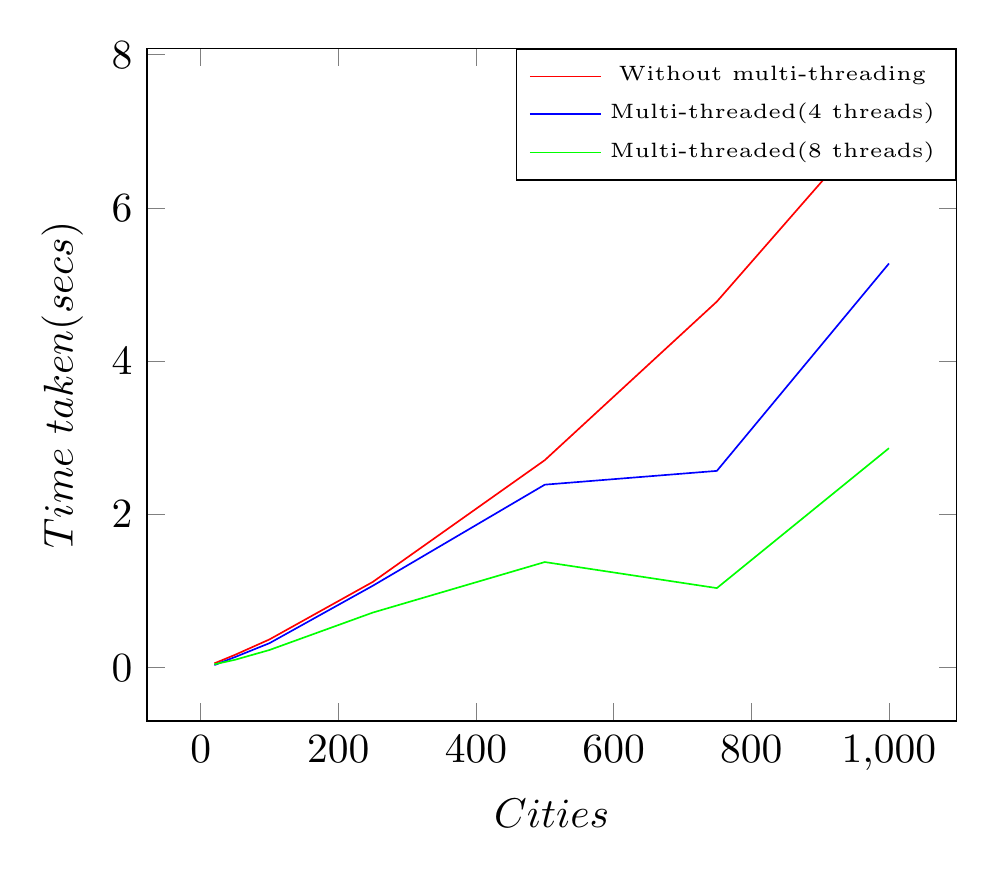
\begin{tikzpicture}[scale=1.5]
		\begin{axis}[
    		legend style={at={(1,1)}, anchor=north east,font=\fontsize{4}{5}\selectfont},
    		xlabel = $Cities$,
    		ylabel = {$Time\ taken(secs)$},
		]
		
		\addplot [
    		color=red,
		]
		coordinates{(20,0.058) (50,0.169) (100,0.37) (250,1.12) (500,2.71) (750,4.78) (1000,7.35)};
		\addlegendentry{Without multi-threading}
		
		\addplot [
    		color=blue,
		]
		%%%%%%%%%%4 threads%%%%%%%%%%%%%%
		coordinates{(20,0.035) (50,0.14) (100,0.3212) (250,1.07) (500,2.39) (750,2.57) (1000,5.277)};
		\addlegendentry{Multi-threaded($4$ threads)}
		
		\addplot [
    		color=green,
		]
		%%%%%%%%%%8 threads%%%%%%%%%%%%%%(find for 20 at last)
		coordinates{(20,0.045) (50,0.1044) (100,0.232) (250,0.72) (500,1.38) (750,1.04) (1000,2.866)};
		\addlegendentry{Multi-threaded($8$ threads)}
 
		\end{axis}
	\end{tikzpicture}
	\end{center}
	\newpage
	\begin{center}
	 \textbf{\textit{generations = 5000}}
	 \end{center}
	 \begin{center}
	 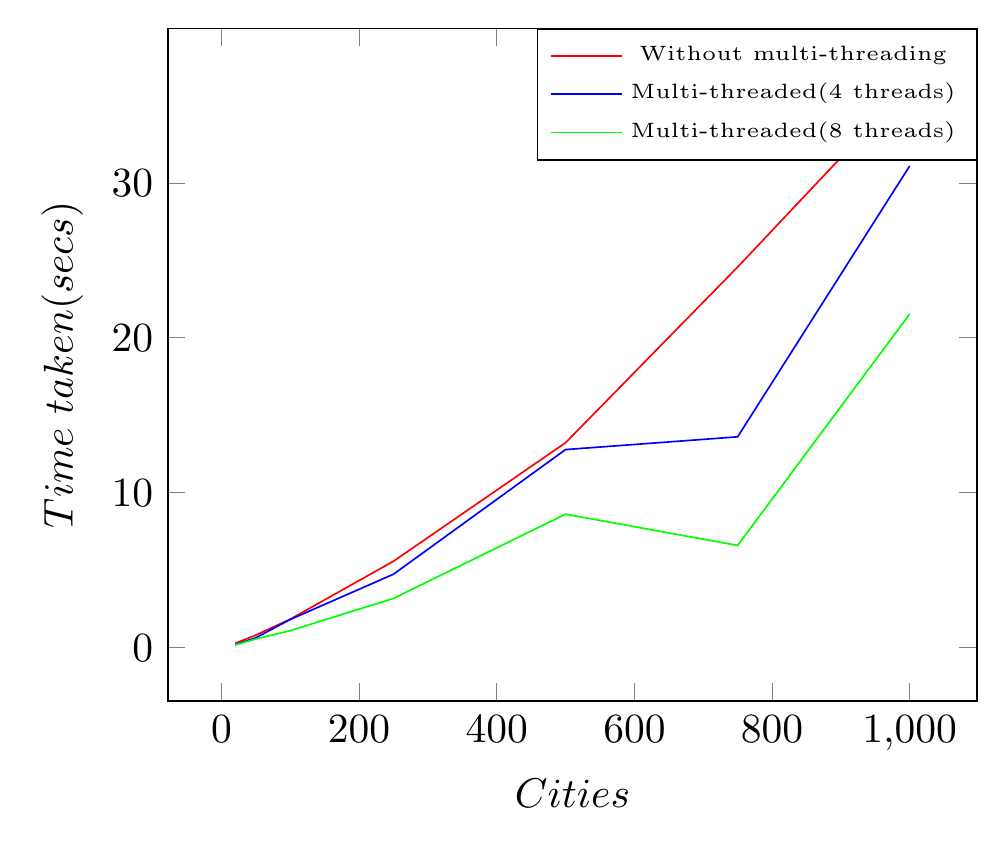
\begin{tikzpicture}[scale=1.5]
		\begin{axis}[
			legend style={at={(1,1)}, anchor=north east,font=\fontsize{4}{5}\selectfont},
    		xlabel = $Cities$,
    		ylabel = {$Time\ taken(secs)$},
		]
		
		\addplot [
    		color=red,
		]
		coordinates{(20,0.28) (50,0.81) (100,1.84) (250,5.58) (500,13.23) (750,24.57) (1000,36.35)};
		\addlegendentry{Without multi-threading}
		
		\addplot [
    		color=blue,
		]
		%%%%%%%%%%4 threads%%%%%%%%%%%%%%
		coordinates{(20,0.19) (50,0.64) (100,1.82) (250,4.742) (500,12.787) (750,13.61) (1000,31.1)};
		\addlegendentry{Multi-threaded($4$ threads)}
		
		\addplot [
    		color=green,
		]
		%%%%%%%%%%8 threads%%%%%%%%%%%%%%
		coordinates{(20,0.1766) (50,0.56) (100,1.10) (250,3.18) (500,8.618) (750,6.6) (1000,21.54)};
		\addlegendentry{Multi-threaded($8$ threads)}
		
 
		\end{axis}
	\end{tikzpicture}
	\end{center}
	\newpage
	\begin{center}
	 \textbf{\textit{generations = 10000}}
	 \end{center}
	 \begin{center}
	 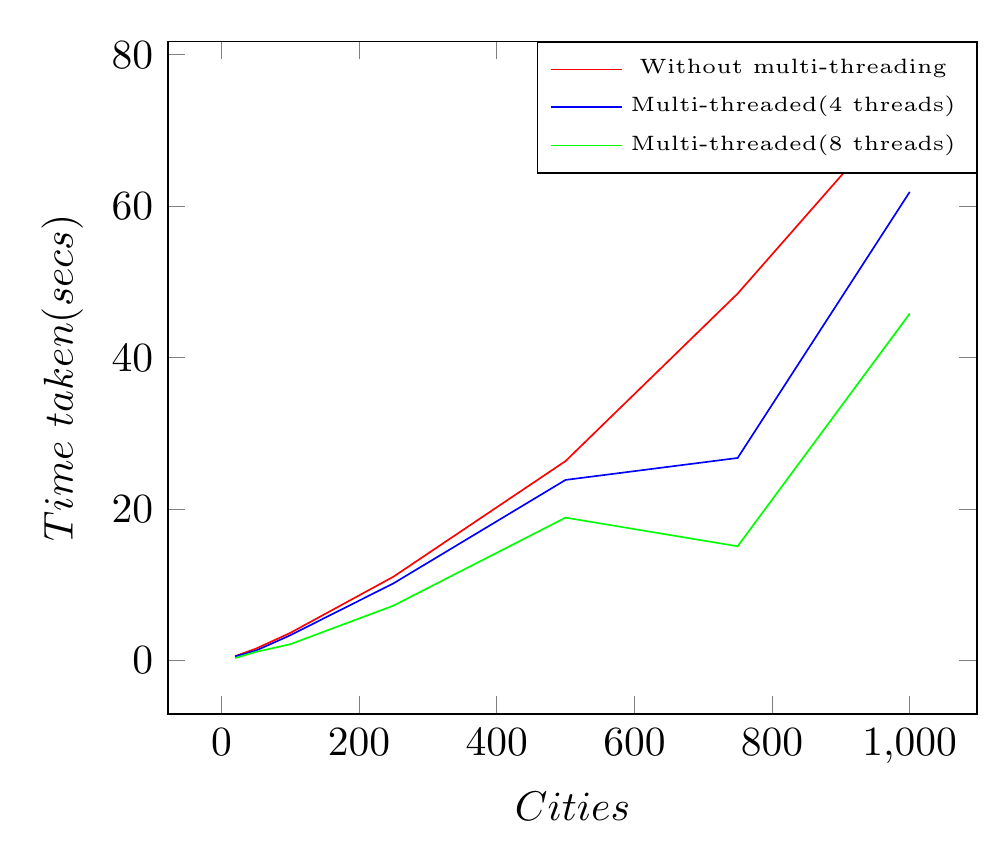
\begin{tikzpicture}[scale=1.5]
		\begin{axis}[
    		legend style={at={(1,1)}, anchor=north east,font=\fontsize{4}{5}\selectfont},
    		xlabel = $Cities$,
    		ylabel = {$Time\ taken(secs)$},
		]
		
		\addplot [
    		color=red,
		]
		coordinates{(20,0.58) (50,1.57) (100,3.65) (250,11.08) (500,26.35) (750,48.47) (1000,74.35)};
		\addlegendentry{Without multi-threading}
		
		\addplot [
    		color=blue,
		]
		%%%%%%%%%%4 threads%%%%%%%%%%%%%%
		coordinates{(20,0.55) (50,1.31) (100,3.34) (250,10.2) (500,23.86) (750,26.76) (1000,61.9)};
		\addlegendentry{Multi-threaded($4$ threads)}
		
		\addplot [
    		color=green,
		]
		%%%%%%%%%%8 threads%%%%%%%%%%%%%%
		coordinates{(20,0.3352) (50,1.1422) (100,2.156) (250,7.2561) (500,18.88) (750,15.1) (1000,45.822)};
		\addlegendentry{Multi-threaded($8$ threads)}
		
 
		\end{axis}
	\end{tikzpicture}
	\end{center}

\end{document}
